\documentclass{beamer}\usepackage[]{graphicx}\usepackage[]{color}
% maxwidth is the original width if it is less than linewidth
% otherwise use linewidth (to make sure the graphics do not exceed the margin)
\makeatletter
\def\maxwidth{ %
  \ifdim\Gin@nat@width>\linewidth
    \linewidth
  \else
    \Gin@nat@width
  \fi
}
\makeatother

\definecolor{fgcolor}{rgb}{0.345, 0.345, 0.345}
\newcommand{\hlnum}[1]{\textcolor[rgb]{0.686,0.059,0.569}{#1}}%
\newcommand{\hlstr}[1]{\textcolor[rgb]{0.192,0.494,0.8}{#1}}%
\newcommand{\hlcom}[1]{\textcolor[rgb]{0.678,0.584,0.686}{\textit{#1}}}%
\newcommand{\hlopt}[1]{\textcolor[rgb]{0,0,0}{#1}}%
\newcommand{\hlstd}[1]{\textcolor[rgb]{0.345,0.345,0.345}{#1}}%
\newcommand{\hlkwa}[1]{\textcolor[rgb]{0.161,0.373,0.58}{\textbf{#1}}}%
\newcommand{\hlkwb}[1]{\textcolor[rgb]{0.69,0.353,0.396}{#1}}%
\newcommand{\hlkwc}[1]{\textcolor[rgb]{0.333,0.667,0.333}{#1}}%
\newcommand{\hlkwd}[1]{\textcolor[rgb]{0.737,0.353,0.396}{\textbf{#1}}}%
\let\hlipl\hlkwb

\usepackage{framed}
\makeatletter
\newenvironment{kframe}{%
 \def\at@end@of@kframe{}%
 \ifinner\ifhmode%
  \def\at@end@of@kframe{\end{minipage}}%
  \begin{minipage}{\columnwidth}%
 \fi\fi%
 \def\FrameCommand##1{\hskip\@totalleftmargin \hskip-\fboxsep
 \colorbox{shadecolor}{##1}\hskip-\fboxsep
     % There is no \\@totalrightmargin, so:
     \hskip-\linewidth \hskip-\@totalleftmargin \hskip\columnwidth}%
 \MakeFramed {\advance\hsize-\width
   \@totalleftmargin\z@ \linewidth\hsize
   \@setminipage}}%
 {\par\unskip\endMakeFramed%
 \at@end@of@kframe}
\makeatother

\definecolor{shadecolor}{rgb}{.97, .97, .97}
\definecolor{messagecolor}{rgb}{0, 0, 0}
\definecolor{warningcolor}{rgb}{1, 0, 1}
\definecolor{errorcolor}{rgb}{1, 0, 0}
\newenvironment{knitrout}{}{} % an empty environment to be redefined in TeX

\usepackage{alltt}
\usepackage{dcolumn}
\usetheme{UMN}

%%%%%%%%%%%%%%%%%%%%%%%%%%%%%%%%%%%%%%%%%%%%%%%%%%%%%%%%%%%%%%%%
% Setup
%%%%%%%%%%%%%%%%%%%%%%%%%%%%%%%%%%%%%%%%%%%%%%%%%%%%%%%%%%%%%%%%%%

% Aaron
% plots with state variation

\title[Felony Records and the U.S. Labor Force]{Felony Records and the Decline in U.S. Labor Force Participation, 1980-2010}

% A subtitle is optional and this may be deleted
\subtitle{}

\author[Larson et. al.]{Ryan Larson \inst{1}, Chris Uggen \inst{1}, Sarah Shannon \inst{2}, Aaron Sojourner \inst{3}}



% - Give the names in the same order as the appear in the paper.
% - Use the \inst{?} command only if the authors have different
%   affiliation.

\institute [UMN, UGA] % (optional, but mostly needed)
{
  \inst{1}
  Department of Sociology, 
  University of Minnesota\\
  \inst{2}
  Department of Sociology, 
  University of Georgia\\
  \inst{3}
  Carlson School of Management, 
  University of Minnesota
 
}

\date{PAA, 2020}


\logo{
 \makebox[0.95\paperwidth]{
    
\includegraphics[width=1cm,height=1cm,keepaspectratio]{umn.png}
      \hfill
    
\includegraphics[width=1cm,height=1cm,keepaspectratio]{uga.png}
}}

% Delete this, if you do not want the table of contents to pop up at
% the beginning of each subsection:
\AtBeginSubsection[]
{
  \begin{frame}<beamer>{Outline}
    \tableofcontents[currentsection,currentsubsection]
  \end{frame}
}

%%%%%%%%%%%%%%%%%%%%%%%%%%%%%%%%%%%%%%%%%%%%%%%%%%%%%%%%%%%%%%%%%%%%%%%%%%%%%%%%%%%%%%%%%%%%%%%%%%%%%%%%%%%%




\IfFileExists{upquote.sty}{\usepackage{upquote}}{}
\begin{document}

%title page
\begin{frame}
  \titlepage
\end{frame}

%outline
\begin{frame}{Outline}
  \tableofcontents
  % You might wish to add the option [pausesections]
\end{frame}

\section{Introduction}

\begin{frame}{Context - Employment}



\begin{knitrout}
\definecolor{shadecolor}{rgb}{0.969, 0.969, 0.969}\color{fgcolor}
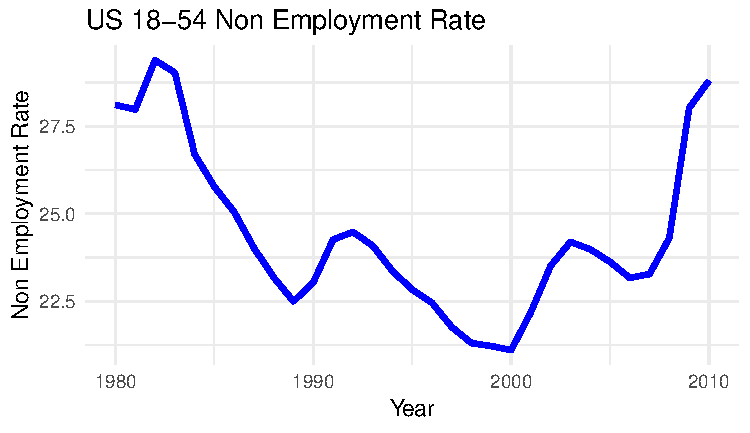
\includegraphics[width=\maxwidth]{figure/unnamed-chunk-2-1} 

\end{knitrout}



\end{frame}

\begin{frame}{Context - Criminal Records}


\begin{knitrout}
\definecolor{shadecolor}{rgb}{0.969, 0.969, 0.969}\color{fgcolor}
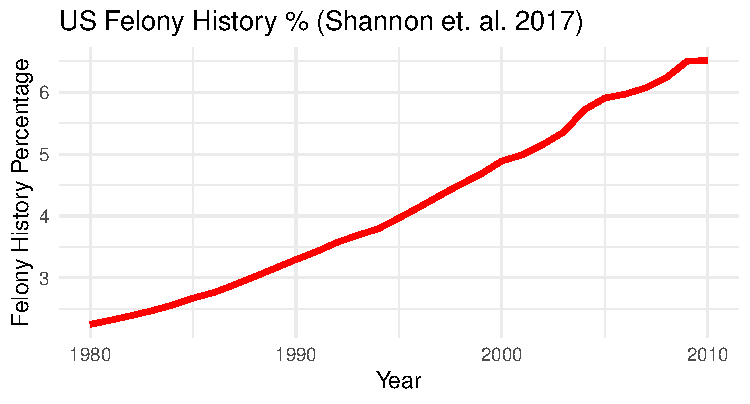
\includegraphics[width=\maxwidth]{figure/unnamed-chunk-3-1} 

\end{knitrout}



\end{frame}

\begin{frame}{Spatial Variation}




\begin{knitrout}
\definecolor{shadecolor}{rgb}{0.969, 0.969, 0.969}\color{fgcolor}
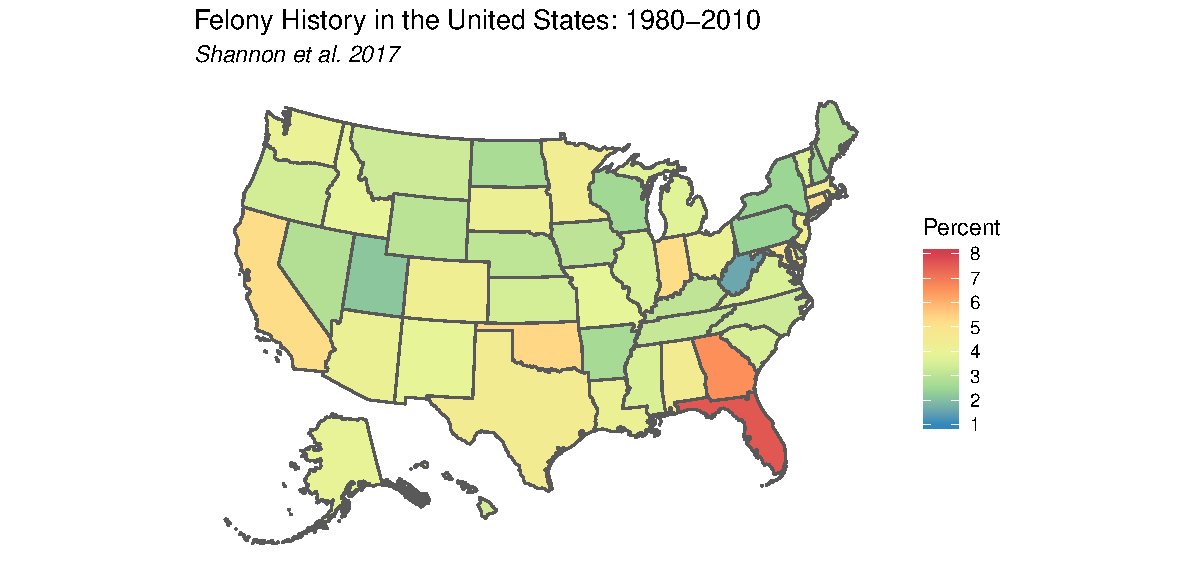
\includegraphics[width=\maxwidth]{figure/unnamed-chunk-5-1} 

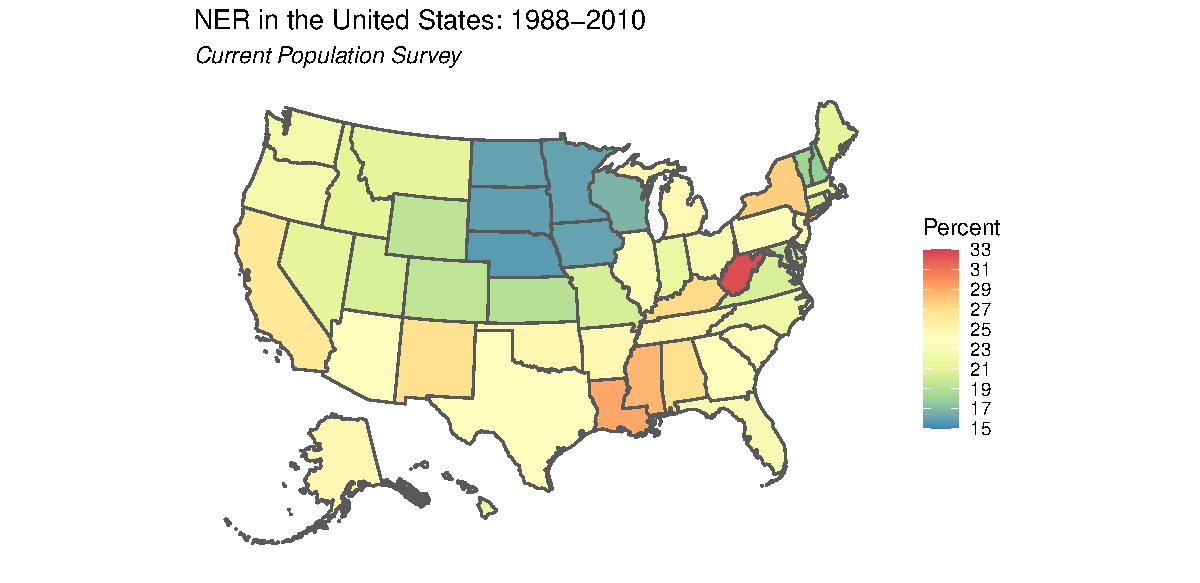
\includegraphics[width=\maxwidth]{figure/unnamed-chunk-5-2} 

\end{knitrout}

\end{frame}

\begin{frame}{State variation in Non Employment}
\begin{knitrout}
\definecolor{shadecolor}{rgb}{0.969, 0.969, 0.969}\color{fgcolor}
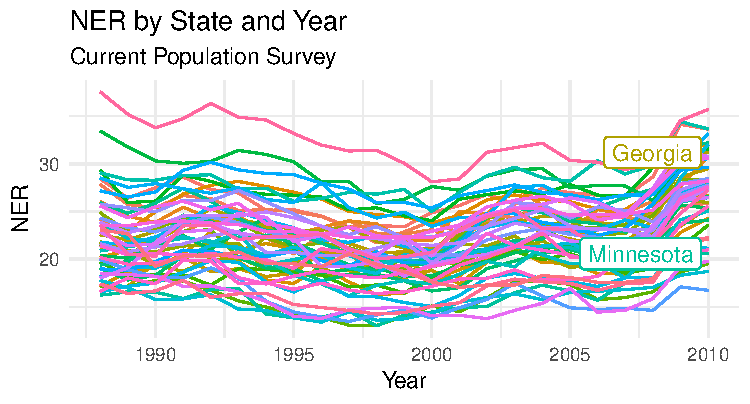
\includegraphics[width=\maxwidth]{figure/unnamed-chunk-6-1} 

\end{knitrout}
\end{frame}

\begin{frame}{State Variation in Felony History}
\begin{knitrout}
\definecolor{shadecolor}{rgb}{0.969, 0.969, 0.969}\color{fgcolor}
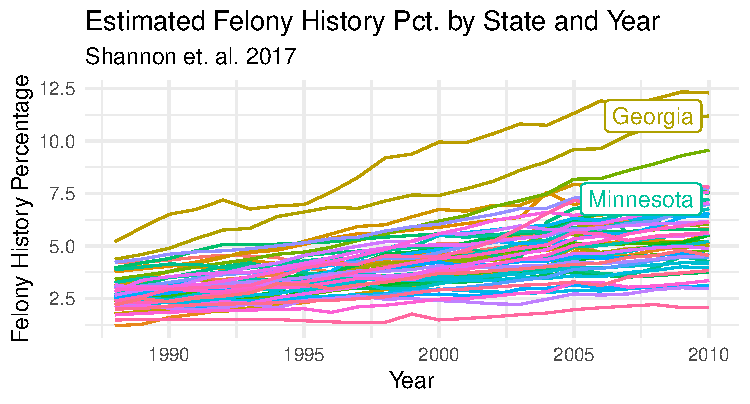
\includegraphics[width=\maxwidth]{figure/unnamed-chunk-7-1} 

\end{knitrout}
\end{frame}

\begin{frame}{Questions}
\begin{block}{}
\begin{itemize}

\item How has the proliferation of criminal record altered chances in the U.S. labor market?

\item Is the effect robust across subpopulations? Chiricos et. al. (2005), Western (2002)

\end{itemize}
\end{block}
\end{frame}

\section{Literature}

\begin{frame}

\begin{block}{Theory}
\begin{itemize}
\item Labeling and Stigma (Goffman 1963, Becker 1963)
\item Age-Graded Life Course (Sampson and Laub 1997)
\item Statistical Discrimination (Arrow 1973) and Signaling (Bushway and Apel 2011)
\end{itemize}
\end{block}

\begin{block}{Empirical}
\begin{itemize}
\item Experimental Audits: Pager (2003), Uggen et. al. (2014)
\item Observational data: Sampson and Laub (1993), Western (2002), Stoll and Bushway (2008), Apel and Sweeten (2010), Harding et. al. (2018)
\item Macro Level: effects range from 0-0.13 (Looney \& Turner 2018, Abraham \& Kearney 2018)
\end{itemize}
\end{block}

\end{frame}

\section{Methods}
\subsection{Data}

\begin{frame}{Data}
\begin{block}{}
\begin{itemize}

\item Balanced Panel of U.S. State-Years 1980-2010 (50*31=1,550 obs.*)
\item Population: U.S. adults ages 18-54 (excludes those incarcerated)
\item Current Population Survey data aggregated to state-year level
\item Merge covariates from UKCPR, CSP, SSA
\item Leverage new state-year estimates of population with felony record (Shannon et. al. 2017)
  \begin{itemize}
  \item estimated via demographic life-tables of correctional out-flows 
  \item adjusts each cohort accounting for mortality and recidivism
  \item excludes those currently under correctional supervision
  \end{itemize}
\end{itemize}
\end{block}
\end{frame}

\subsection{Measures}

\begin{frame}{Measures}
\begin{block}{Outcome Measures}
\begin{itemize}

\item DV: not employed share (unemployed+NILF)/population 
\item IV: felony history percentage
\item Time-Varying Controls:
  \begin{itemize}
  \item Population age shares
  \item Overall unemployment rate lags (proxies for business cycle)
  \item Disability, marriage, and bachelor's degree rates
  \item Effective wage, unemployment compensation, mean TANF max
\end{itemize}

\end{itemize}
\end{block}
\end{frame}

\subsection{Analytical Strategy}


\begin{frame}{Analytical Strategy}
\begin{block}{Generalized Difference-in-Difference}
\begin{itemize}
\item "treatment" as dosage of felony history
\item assumes units would follow a common employment trajectory with equivalent doses
\item modeled as a "two-way" fixed effects panel model
\item $Y_{st} = \beta F_{st} + \alpha X_{st} + \lambda_s + \lambda_t + \epsilon_{st}$
\item stable, unobserved influences across states and years captured by fixed effects
\item causal if*: unobserved within state changes, not due to common time shocks, independent of changes in $F_{st}$
\item cluster SEs by state and year
  \begin{itemize}
  \item state: heteroskedasticity and autocorrelation across time within state
  \item year: spatial autocorrelation within year
  \end{itemize}

\end{itemize}
\end{block}
\end{frame}



\section{Results}




\begin{frame}{Overall FE Model}


\begin{table}[!htbp] \centering 
  \caption{Panel Model of Not Employed Rate, 1988-2010} 
  \label{} 
\small 
\begin{tabular}{@{\extracolsep{1pt}}lD{.}{.}{-2} } 
\\[-1.8ex]\hline 
\hline \\[-1.8ex] 
\hline \\[-1.8ex] 
 Felony History Pct. & 0.33$ $(0.11)^{**} \\ 
  Disab. Rate & 0.15$ $(0.05)^{**} \\ 
  Marriage Rate & 0.01$ $(0.04) \\ 
  Effective Wage & -0.05$ $(0.13) \\ 
  Mean TANF Maximum & 0.00$ $(0.00) \\ 
  Unemployment Comp. & -0.00$ $(0.00) \\ 
  Degree Rate & -0.05$ $(0.04) \\ 
 State FE & Yes \\ 
Year FE & Yes \\ 
\hline \\[-1.8ex] 
\textit{Notes:} & \multicolumn{1}{l}{$^{***}$Significant at the 0.1 percent level.} \\ 
 & \multicolumn{1}{l}{$^{**}$Significant at the 1 percent level.} \\ 
 & \multicolumn{1}{l}{$^{*}$Significant at the 5 percent level.} \\ 
\end{tabular} 
\end{table} 


\end{frame}


\begin{frame}



\begin{knitrout}
\definecolor{shadecolor}{rgb}{0.969, 0.969, 0.969}\color{fgcolor}
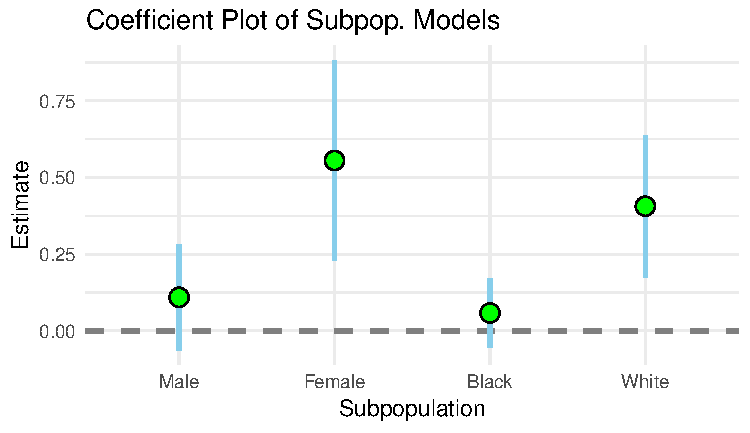
\includegraphics[width=\maxwidth]{figure/unnamed-chunk-11-1} 

\end{knitrout}
\end{frame}


\section{Summary}

\begin{frame}{Summary}
\begin{block}{Conclusions}
\begin{itemize}
\item collateral consequences do move the needle in aggregate employment
\item but only for females and whites; effects vs. levels
\item consistent with Chiricos et. al. 2005
\end{itemize}
\end{block}

\begin{block}{Limitations and future research}
\begin{itemize}
\item causal identification: threat of time-varying unmeasured idiosyncrasies
\item do not have sub population specific IV at state-year level
\item further work leverage exogenous policy change to indentify effect (e.g., truth in sentencing)
\end{itemize}
\end{block}
\end{frame}

\begin{frame}{Questions/Comments?}

\begin{block}

\item Ryan Larson
\item Email: lars3965@umn.edu
\item Twitter: @ryanplarson

\end{block}

\end{frame}



\begin{frame}{Appendix: Rolling Window Estimates}



\begin{knitrout}
\definecolor{shadecolor}{rgb}{0.969, 0.969, 0.969}\color{fgcolor}
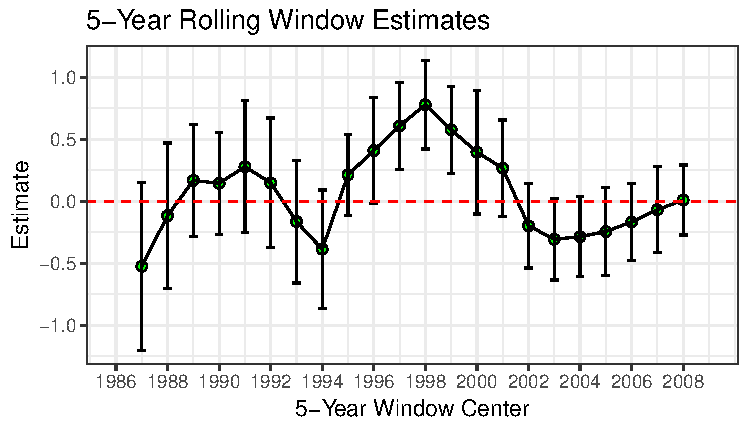
\includegraphics[width=\maxwidth]{figure/unnamed-chunk-13-1} 

\end{knitrout}


\end{frame}




\end{document}





